\chapter{Théorie des graphes}
\section{Définitions et concept fondamental (graphe non orienté)}
\subsection{Définitions}
\noindent De façon conceptuelle, un graphe est formé par des sommets (Vertices en anglais) et des arêtes (Edges en anglais) 
qui relient les sommets entre-eux.

\begin{figure}[h]
\centering
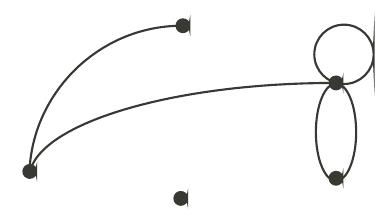
\includegraphics[width=0.5\linewidth]{images/graph}
\caption[Exemple d'un graphe]{Exemple de graphe}
\label{fig:graph}
\end{figure}

\noindent En d'autre terme, un \textbf{graphe} fini noté $G=(V,E)$ est défini par l'ensemble fini $V\ = \{v_{1},\ v_{2},\dots,\ v_{n} \}$ 
dont les éléments sont appelés \textbf{sommets}, 
et par un ensemble fini 
$ E\ = \{ e_{1},\ e_{2},\dots ,\ e_{m} \} $
dont les éléments sont appelés \textbf{arêtes}.

\noindent Une arête $ e $ de l'ensemble $ E $ est définie par une paire non ordonnée de sommets, appelés
les \textbf{extrémités} de $ e $. Si l'arête $ e $ relie les sommets $ u $ et $ v $, on note $ e=\ (u,v) $, on dira que ces sommets sont
\textbf{adjacents}, ou \textbf{incidents} avec $ e $, ou bien que l'arête $ e $ est incidente avec 
les sommets $ u $ et $ v $.\\
Des arêtes sont adjacentes si elle partagent les mêmes extrémités.
On appelle \textbf{ordre} d'un graphe le nombre de sommets n de ce graphe.\\
Les arêtes sont dites \textbf{parallèle} s'ils ont les mêmes extrémités. \\
On appelle \textbf{boucle} l'arête $ e $ de la forme $ (u,u) $. \\
On dit qu'un graphe est un \textbf{graphe simple} s'il ne possède pas des arêtes parallèle et de boucle. \\
Un graphe sans arêtes (c'est-à-dire $E$ est vide )est \textbf{vide}.\\
Un graphe sans sommets (c'est-à-dire $V$ et $E$ sont vides) est un \textbf{graphe nul}.\\
Un graphe avec un seul sommet est dit \textbf{trivial}.\\
Le degré d'un sommet $v$, noté $d(v)$, est le nombre des arêtes qui parent du sommet $v$.
Par convention, une boucle compte deux fois et les arêtes parallèles sont comptées séparément.
Un sommet isolé est un sommet qui a un degré nul.


\begin{figure}[ht]
\centering
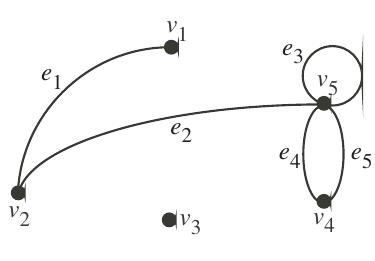
\includegraphics[width=0.5\linewidth]{images/graph1}
\caption[Étiquetage des sommets et des arêtes]{Étiquetage des sommets et des arêtes}
\label{fig:graph1}
\end{figure} 
\paragraph*{}
En prenant l'exemple du Fig. \ref{fig:graph1}:
\begin{itemize}
	\item[\textbullet] $v_{4}$ et $v_{5}$ sont les extrémités de $e_{5}$.
	\item[\textbullet] $e_{4}$ et $e_{5}$ sont parallèle.
	\item[\textbullet] $e_{3}$ est une boucle.
	\item[\textbullet] Ce graphe n'est pas simple.
	\item[\textbullet] $e_{1}$ et $e_{2}$ sont adjacents.
	\item[\textbullet] $v_{1}$ et $v_{2}$ sont adjacentes.
	\item[\textbullet] Le degré du sommet $v_{5}$ est 5.
	\item[\textbullet] Le degré du sommet $v_{4}$ est 2.
	\item[\textbullet] Le degré du sommet $v_{3}$ est 0 donc le sommet est isolé.
\end{itemize}

On note $\delta (G)$ (respectivement $\varDelta (G)$) le degré minimum (respectivement maximum)
des sommets dans le graphe G.
En prenant toujours l'exemple précédent,  $\delta (G) = 0$ et $\varDelta (G) = 5$.
\paragraph*{Remarque.} Dans ce rapport, on considère seulement les graphes finis, c'est-à-dire
$V$ et $E$ sont des ensembles finis.

Comme chaque arêtes ont deux extrémités, on a:

\paragraph*{Théorème 1.1.} Le graphe $G=(V,E)$, où $V = \{v_{1},\dots,v_{n}\}$ et
$E=\{e_{1},\dots,e_{m} \}$, donne
	$$ \sum_{i=1}^{n}d(v_{i})\ =\ 2m  $$
\paragraph*{Corolaire 1.2.} Chaque graphe a un nombre pair de sommets d'un degré impair.

\paragraph*{\textit{Preuve.}} Si les sommets $v_{1},\dots,v_{k}$ ont un degré impair et 
les sommets $v_{k+1},\dots,v_{n}$ ont un degré pair, alors (Théorème 1.1.)
$$ d(v_{1}+\dots +v_{k}=2m -\ d(v_{k+1})\ -\ \dots-d(v_{n})$$ 
est pair. D'où, k pair.

En prenant encore l'exemple précédent, la somme des degrés est $ 1+2+0+2+5 = 10 = 2\times 5$.
Il y a deux sommets d'un degré pair qui sont $v_{1}$ et $v_{5}$.

\paragraph*{}
Un graphe est dit \textit{graphe complet} chaque sommet du graphe est relié directement à tous les autres
sommets.
Un graphe complet avec $n$ sommets est noté $K_{n}$. Les quatre premiers graphes complets sont donnés
par Fig.\ref{fig:graph2}. 

\begin{figure}[h]
\centering
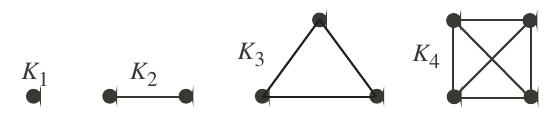
\includegraphics[width=0.5\linewidth]{images/graph2}
\caption[Les quatre premiers graphes complets.]{Les quatre premiers graphes complets.}
\label{fig:graph2}
\end{figure}
\paragraph*{}
\noindent Le graphe $G_{1} = (V_{1},E_{1})$ est un sous-graphe de $G_{2}=(V_{2},E_{2})$ si:
\begin{itemize}
	\item[1.] $V_{1}\subseteq V_{2}$ et
	\item[2.] Chaque arête de $G_{1}$ est aussi une arête de $G_{2}$.
\end{itemize}

\paragraph*{Autres types de graphes}.\\
On appelle \textbf{multigraphes} tous les graphes qui contiennent une boucle, ou
plusieurs arêtes reliant les deux mêmes sommets.

\begin{figure}[h]
\centering
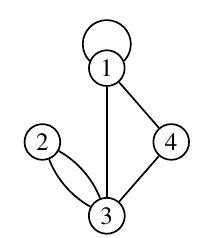
\includegraphics[width=0.2\linewidth]{images/graph3}
\caption[Multigraphe.]{Multigraphe.}
\label{fig:graph3}
\end{figure}

Un graphe est \textbf{connexe} s'il est possible à partir de n'importe quel sommet,
de rejoindre tous les autres en suivant les arêtes. Un graphe non connexe se décompose en composantes
connexes. Sur le graphe ci-dessous, les composantes connexes sont {1, 2, 3, 4} et {5, 6}.
 
\begin{figure}[h]
\centering
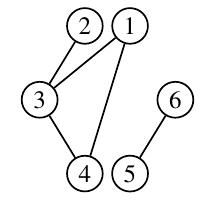
\includegraphics[width=0.2\linewidth]{images/graph4}
\caption[Graphe connexe.]{Graphe connexe.}
\label{fig:graph4}
\end{figure}

Un graphe est \textbf{biparti} si ses sommets peuvent être divisés en deux ensembles X et Y ,
de sorte que toutes les arêtes du graphe relient un sommet dans X à un sommet dans Y
(dans l'exemple ci-dessous, on a X = {1, 3, 5} et Y = {2, 4}, ou vice versa).

\begin{figure}[h]
\centering
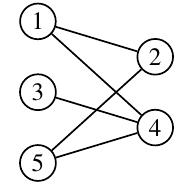
\includegraphics[width=0.2\linewidth]{images/graph5}
\caption[Graphe biparti.]{Graphe biparti.}
\label{fig:graph5}
\end{figure}

\newpage
\subsection{Chaînes et cycles}
\noindent Une \textbf{chaîne} dans G, est une suite ayant pour éléments alternativement des sommets et des
arêtes, commençant et se terminant par un sommet, et telle que chaque arête est encadrée
par ses extrémités.
\paragraph*{}
\noindent On dira que la chaîne \textbf{relie} le premier sommet de la suite au dernier sommet. En plus, on
dira que la chaîne a pour longueur le nombre d'arêtes de la chaîne.

\begin{figure}[h]
\centering
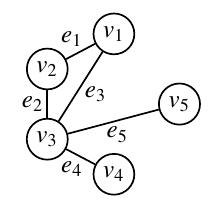
\includegraphics[width=0.2\linewidth]{images/graph6}
\caption[Chaîne.]{Le graphe G contient entre autres les chaînes $ (v_{1} , e_{1} , v_{2} , e_{2} , v_{3} , e_{5} , v_{5} ) $
	et $ (v_{4} , e_{4} , v_{3} , e_{2} , v_{2} , e_{1} , v_{1} ) $.}
\label{fig:graph6}
\end{figure}

\paragraph*{}
\noindent On ne change pas une chaîne en inversant l'ordre des éléments dans la suite correspondante.
Ainsi, les chaînes $ (v_{1} , e_{3} , v_{3} , e_{4} , v_{4} ) $ et
 $ (v_{4} , e_{4} , v_{3} , e_{3} , v_{1} )$ sont identiques.
 
\paragraph*{Théorème 1.3.} Un graphe est biparti si et seulement s’il ne contient aucun cycle de longueur impaire.

\paragraph*{Théorème 1.4.} Pour un graphe $ G $ ayant $ m $ arêtes, $ n $ sommets et $ p $ composantes connexes, on définit :
$$ \nu (G) =m-n+p$$
$ \nu (G) $ est appelé le nombre \textbf{cyclomatique}. Prononcer " nu de G ".
On a $ \nu (G) \geq  0$ pour tout graphe $ G $.
De plus, $ \nu (G) = 0 $ si et seulement si $ G $ est sans cycle.

\subsection{Graphes eulériens}
On appelle \textbf{cycle eulérien} d'un graphe $ G $ un cycle passant une et une seule fois par chacune
des arêtes de $ G $. Un graphe est dit \textbf{eulérien} s'il possède un cycle eulérien.
On appelle \textbf{chaîne eulérienne} d'un graphe G une chaîne passant une et une seule fois par
chacune des arêtes de G. Un graphe ne possédant que des chaînes eulériennes est \textbf{semi-
eulérien}.
Plus simplement, on peut dire qu'un graphe est eulérien (ou semi-eulérien) s'il est possible
de dessiner le graphe sans lever le crayon et sans passer deux fois sur la même arête.

\subsection{Graphes hamiltoniens}
On appelle \textbf{cycle hamiltonien} d'un graphe G un cycle passant une et une seule fois par
chacun des sommets de G. Un graphe est dit \textbf{hamiltonien} s'il possède un cycle hamiltonien.
On appelle \textbf{chaîne hamiltonienne} d'un graphe G une chaîne passant une et une seule fois
par chacun des sommets de G. Un graphe ne possédant que des chaînes hamiltoniennes est
\textbf{semi-hamiltonien}.
Contrairement aux graphes eulériens, il n'existe pas de caractérisation simple des graphes\\
(semi-)hamiltoniens. On peut énoncer quelques propriétés et conditions suffisantes :
\begin{itemize}
	\item un graphe possédant un sommet de degré 1 ne peut pas être hamiltonien ;
	\item si un sommet dans un graphe est de degré 2, alors les deux arêtes incidentes à ce sommet
	doivent faire partie du cycle hamiltonien ;
	\item les graphes complets $ K_{n} $ sont hamiltoniens.
\end{itemize}

\paragraph*{Théorème 1.5.(Ore)} Soit $G$ un graphe simple d'ordre $n\geq 3$. Si pour toute paire $\{x,y\}$ 
de sommets non adjacents, on a $d(x) + d(y) \geq n$, alors $G$ est hamiltonien.

\paragraph*{Corollaire 1.6.(Dirac)} Soit $G$ un graphe simple d'ordre $n\geq 3$. Si pour tout sommet $x$ de $G$,
on a $d(x) \geq \dfrac{n}{2}$, alors $G$ est hamiltonien.

\subsection{Couplages}
Soit $ G $ un graphe simple. Un \textbf{couplage} $ C $ de $ G $ est un sous-graphe partiel 1-régulier de $ G$.
On peut aussi dire qu'un couplage (ou appariement) est un ensemble d'arêtes deux à deux
non-adjacentes.
Un sommet $ v $ est \textbf{saturé} par un couplage $ C $ si $ v $ est l'extrémité d'une arête de $ C $ . Dans le
cas contraire, $ v $ est \textbf{insaturé}.
Un couplage maximum est un couplage contenant le plus grand nombre possible d'arêtes.
Un graphe peut posséder plusieurs couplages maximum.

\begin{figure}[h]
\centering
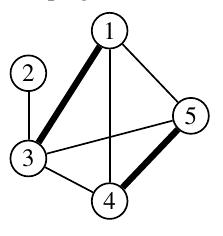
\includegraphics[width=0.3\linewidth]{images/graph8}
\caption{En gras, un couplage maximum de G. Les sommets 1, 3, 4 et 5 sont saturés.}
\label{fig:graph8}
\end{figure}

Un \textbf{couplage parfait} est un couplage où chaque sommet du graphe est saturé.

\begin{figure}[h]
\centering
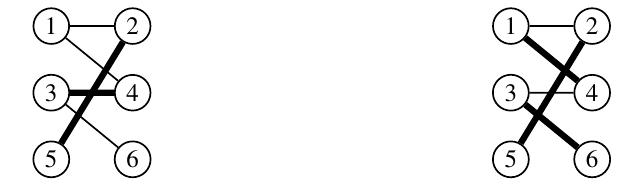
\includegraphics[width=0.7\linewidth]{images/graph9}
\caption{Un couplage (à gauche); Un couplage maximum et parfait (à droite)}
\label{fig:graph9}
\end{figure}

\paragraph*{Calcule d'un couplage maximum }
Si $ C $ est un couplage de $ G $, on appelle \textbf{chaîne alternée} une chaîne élémentaire de \textbf{G} dont
les arêtes sont alternativement dans $ C $ et hors de $ C $.
Une chaîne alternée est dite augmentante si elle relie deux sommets insaturés. Ci-dessus,
à gauche, la chaîne 1-4-3-6 est augmentante. En "intervertissant les épaisseurs" des arêtes
le long de cette chaîne, on obtient un meilleur couplage (ci-dessus, à droite).

\paragraph*{Théorème 1.7.(Berge, 1957)} Un couplage $ C $ est maximum si et seulement 
s'il n'existe pas de chaîne augmentante
relativement à $ C $.


\subsection{Graphes planaires}
On dit qu'un graphe est \textbf{planaire} si on peut le dessiner dans le plan de sorte que ses arêtes
ne se croisent pas. Rappelons que les arêtes ne sont pas forcément rectilignes.
Une \textbf{carte}, ou graphe \textbf{planaire topologique}, est une représentation particulière d'un multigraphe 
planaire fini. On dit qu'une carte est connexe si son graphe l'est. Une carte divise
le plan en plusieurs régions.
Par exemple, la carte ci-dessous, avec sept sommets et neuf arêtes, divise le plan en quatre
régions $(A, B,C, D)$. Trois régions sont limitées alors que la quatrième $(D)$, extérieure au
diagramme, ne l'est pas.

\begin{figure}[h]
\centering
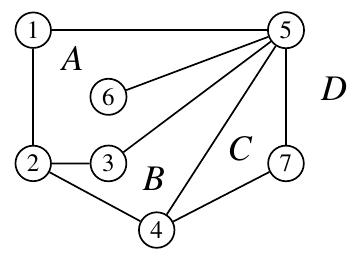
\includegraphics[width=0.4\linewidth]{images/graph10}
\label{fig:graph10}
\end{figure}
\paragraph*{}
\textbf{Le degré d'une région r} , noté $ d(r) $, est la longueur de la chaîne fermée minimum passant 
par tous les sommets qui délimitent cette région. Dans le graphe ci-dessus, $ d(A) = 6 $\\
(la région $ A $ est délimitée par la chaîne fermée passant par les sommets $ (1, 2, 3, 5, 6, 5, 1) $),
$ d(B) = 4 $, $ d(C) = 3 $ et $ d(D) = 5 $.
On remarque que toute arête limite deux régions, ou est contenue dans une région et est
alors comptée deux fois dans la chaîne fermée. Nous avons donc un lemme pour les régions,
analogue au lemme des poignées de mains pour les sommets.

\paragraph*{Théorème 1.8.} La somme des degrés des régions d'une carte connexe est 
égale à deux fois le nombre d'arêtes.

\paragraph*{Théorème 1.9.(Euler 1752)}
Euler a établi une formule célèbre qui relie le nombre de sommets $ S $, le nombre
d'arêtes $ A $ et le nombre de régions $ R $ d'une carte connexe:
$$ S-A+R=2 $$

\paragraph*{Théorème 1.10 (Kuratowski, 1930)}Un graphe est non planaire si et seulement s'il contient 
un sous-graphe homéomorphe (voir lexique) au graphe biparti $ K_{3,3} $ ou au graphe complet $ K_{5} $.

\begin{figure}[h]
\centering
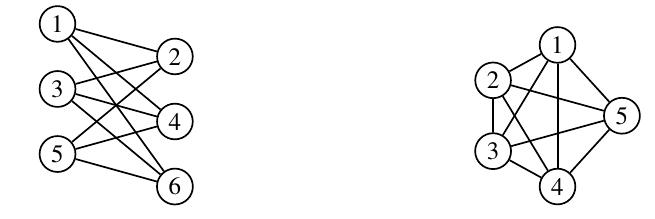
\includegraphics[width=0.7\linewidth]{images/graph11}
\label{fig:graph11}
\end{figure}

\newpage
\subsection{Représentations non graphiques d'un graphe}
\subsubsection{Matrice d'adjacents}
\noindent On peut représenter un graphe simple par une matrice d'adjacences. Une matrice $ (n\times m) $
est un tableau de $ n $ lignes et $ m$  $ $ colonnes. $(i, j)$ désigne l'intersection de la ligne $ i$ et de
la colonne j. Dans une matrice d'adjacences, les lignes et les colonnes représentent les
sommets du graphe. Un $ "1" $  $ $ à la position $ (i, j) $ signifie que le sommet $ i $ est adjacent au
sommet $ j $.

\begin{figure}[h]
\centering
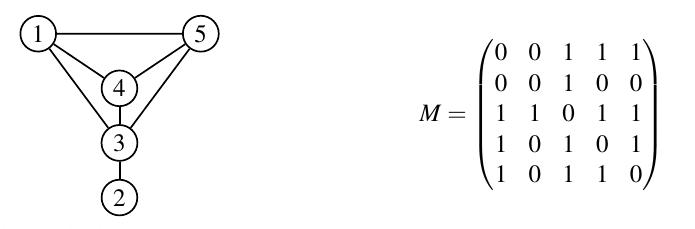
\includegraphics[width=0.7\linewidth]{images/graph7}
\caption[Exemple d'un graphe (à gauche) et sont matrice d'adjacents (à droite).]{Exemple d'un graphe (à gauche) et sont matrice d'adjacents (à droite).}
\label{fig:graph7}
\end{figure}
\paragraph*{}
Cette matrice a plusieurs caractéristiques :

\begin{itemize}
	\item[1.] Elle est carrée : il y a autant de lignes que de colonnes.
	\item[2.] Il n'y a que des zéros sur la diagonale allant du coin supérieur gauche au coin inférieur droit. 
	Un $ "1" $ sur la diagonale indiquerait une boucle.
	\item[3.] Elle est symétrique : $ m_{i j} = m_{ ji} $ . On peut dire que la diagonale est un axe de symétrie.
	\item[4.] Une fois que l'on fixe l'ordre des sommets, il existe une matrice d'adjacences unique
pour chaque graphe. Celle-ci n'est la matrice d'adjacences d'aucun autre graphe.
\end{itemize}
\newpage
\subsubsection{Listes d’adjacences}
\noindent On peut aussi représenter un graphe simple en donnant pour chacun de ses sommets la liste
des sommets auxquels il est adjacent. Ce sont les $ listes d'adjacences $.

\begin{figure}[h]
\centering
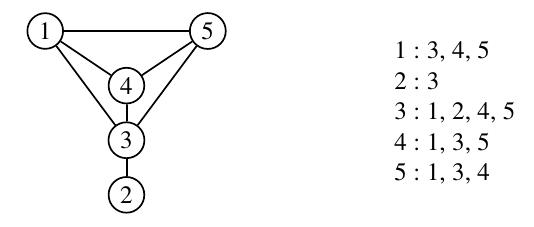
\includegraphics[width=0.7\linewidth]{images/graph12}
\label{fig:graph12}
\end{figure}


\subsection{Arbres}
On appelle \textbf{arbre} tout graphe connexe sans cycle. Un graphe sans cycle mais non connexe
est appelé une \textbf{forêt}.
Une \textbf{feuille} ou \textbf{sommet pendant} est un sommet de degré 1.

\begin{figure}[h]
\centering
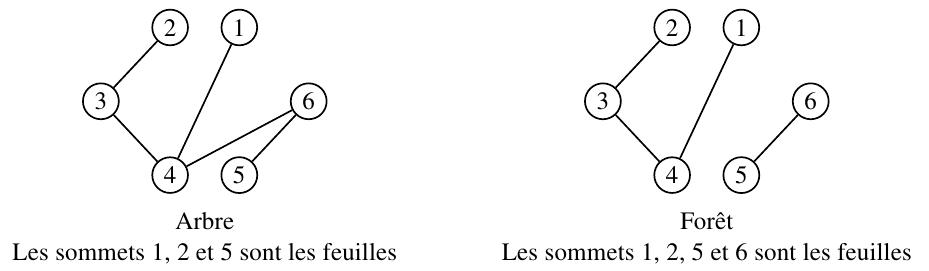
\includegraphics[width=0.7\linewidth]{images/graph13}
\label{fig:graph13}
\end{figure}

\paragraph*{Théorème 1.11.}
Les affirmations suivantes sont équivalentes pour tout graphe G à n sommets.
\begin{itemize}
	\item[1.] $ G $ est un arbre,
	\item[2.] $ G $ est sans cycle et connexe,
	\item[3.] $ G $ est sans cycle et comporte $ n - 1 $ arêtes,
	\item[4.] $ G $ est connexe et comporte $ n - 1 $ arêtes,
	\item[5.] chaque paire $ u,\ v $ de sommets distincts est reliée par une seule chaîne simple (et
	le graphe est sans boucle).
\end{itemize}

\paragraph*{Théorème 1.12.}
Tout arbre fini avec au moins deux sommets comporte au moins deux sommets
pendants.

\subsubsection*{Codage de Prüfer\\}
Le codage de Prüfer (1918) est une manière très compacte de décrire un arbre. Il a été
proposé par le mathématicien allemand Ernst Paul Heinz Prüfer (1896-1934).

\subsubsection*{Codage\\}
Soit l'arbre $ T = (V, E) $ et supposons $ V = \{1, 2, . . . , n \}. $
L'algorithme ci-dessous fournira le code de $ T $ , c'est-à-dire une suite $ S $ de $ n - 2 $ termes
employant (éventuellement plusieurs fois) des nombres choisis parmi $ 1,\dots , n $.
\subsubsection*{Pas général de l'algorithme de codage}
(à répéter tant qu'il reste plus de deux sommets dans l'arbre $ T $ )

\begin{itemize}
	\item[1.] identifier la feuille $ v $ de l'arbre ayant le numéro minimum ;
	\item[2.] ajouter à la suite $ S $ le seul sommet s adjacent à v dans l'arbre $ T $ ;
	\item[3.] enlever de l'arbre $ T $ le sommet $ v $ et l'arête incidente à $ v $.
\end{itemize}

\subsubsection*{Exemple de codage}
\begin{figure}[h]
\centering
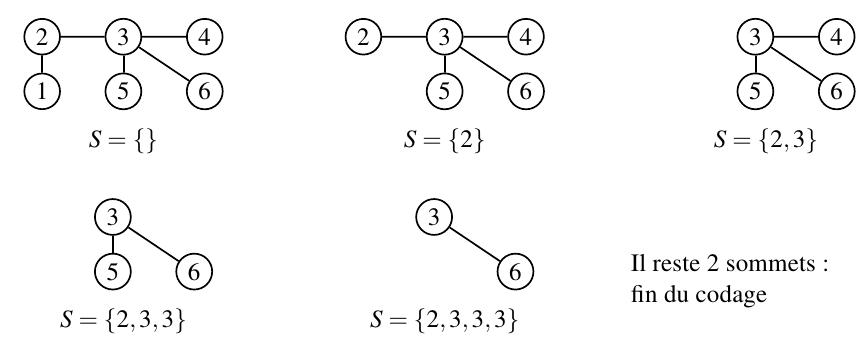
\includegraphics[width=\linewidth]{images/graph14}
\end{figure}

\subsubsection*{Décodage}
Donnée : suite $ S $ de $ n - 2 $ nombres, chacun provenant de $ \{1, \dots , n\} $.
Posons $ I = \{1, \dots , n\} $.
\subsubsection*{Pas général de l'algorithme de décodage}
(à répéter tant qu'il reste des éléments dans $ S $ et plus de deux éléments dans $ I $ )
\begin{itemize}
	\item[1.] identifier le plus petit élément $ i $ de $ I $ n'apparaissant pas dans la suite $ S $ ;
	\item[2.] relier par une arête de $ T $ le sommet $ i $ avec le sommet $ s $ correspondant au premier
élément de la suite $ S $ ;
	\item[3.] enlever $ i $ de $ I $ et $ s $ de $ S $.
\end{itemize}
Les deux éléments qui restent dans $ I $ à la fin de l'algorithme constituent les extrémités de
la dernière arête à ajouter à $ T $ .
\newpage
\subsubsection*{Exemple de décodage}
\begin{figure}[h]
\centering
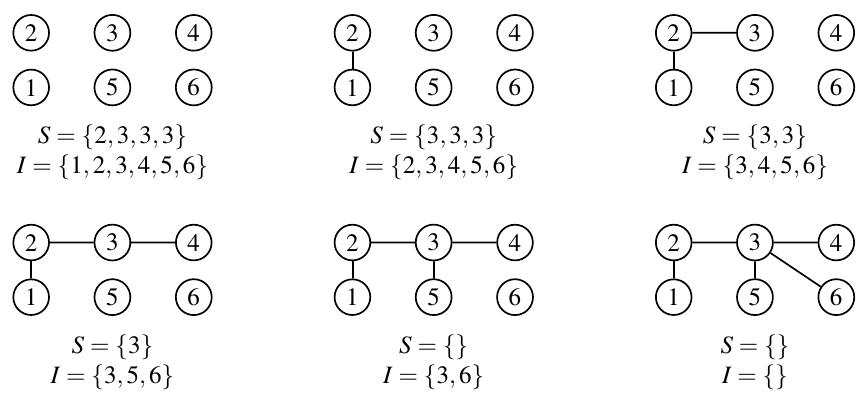
\includegraphics[width=1\linewidth]{images/graph15}
\end{figure}

\paragraph*{Théorème 1.13 (Cayley, 1857)}
Le nombre d'arbres que l'on peut construire sur $ n $ $ (n \geq 2) $ sommets numérotés est
égal à $ n^{n-2} $.

\subsection{Arbres couvrants}
Un \textbf{arbre couvrant} (aussi appelé arbre maximal) est un graphe partiel qui est aussi un
arbre.

\begin{figure}[h]
\centering
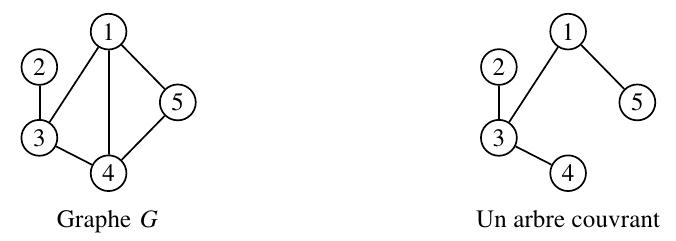
\includegraphics[width=0.7\linewidth]{images/graph16}
\end{figure}

\subsubsection{Arbre couvrant de poids minimum}
Soit le graphe $ G = (V, E) $ avec un poids associé à chacune de ses arêtes. On veut trouver,
dans $ G $, un arbre maximal $ A = (V, F) $ de poids total minimum.

\subsubsection*{Algorithme de Kruskal (1956)}
Données :
\begin{itemize}
	\item Graphe $ G = (V, E) (\textbar V \textbar = n, \textbar E \textbar = m) $
	\item Pour chaque arête e de $ E $ , son poids $ c(e) $.
\end{itemize}
\textit{Résultat} : Arbre ou forêt maximale A = (V, F) de poids minimum.

Trier et renuméroter les arêtes de $ G $ dans l'ordre croissant de leur poids :
$$ c(e_{1} ) \leq c(e_{2} ) \leq \dots \leq c(e_{m}) $$.


\begin{algorithm}
	\caption{Algorithme de Kruskal}\label{euclid}
	\begin{algorithmic}[1]
		\Procedure{}{}
		\State Poser $ F := \varnothing, k := 0 $
		\While {$ k < m $ \textbf{and} $ \textbar F\textbar < n - 1 $}
		\If {$ e_{k}+1 $ ne forme pas de cycle avec $ F $}
		\State$ F := F \bigcup {e_{k+1} } $;
		\EndIf 
		\State $k := k + 1 $;
		\EndWhile
		\EndProcedure
	\end{algorithmic}
\end{algorithm}

\subsection*{Exemple}

\begin{figure}[h]
\centering
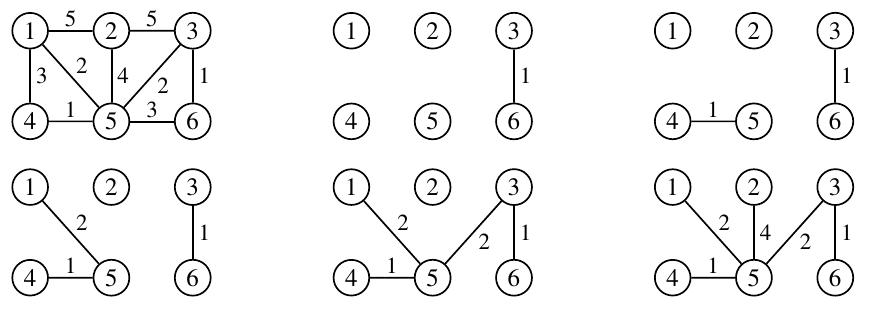
\includegraphics[width=\linewidth]{images/graph17}
\end{figure}

Les arêtes de poids 3 n'ont pas pu être placées, car elles auraient formé un cycle.
L'algorithme s'est arrêté dès que cinq arêtes ont été placées. Toute arête supplémentaire
aurait créé un cycle.
S'il y a plusieurs arêtes de même poids, il peut y avoir plusieurs arbres couvrants de poids
minimum : tout dépend de l'ordre dans lequel ces arêtes ont été triées.

\subsection{Coloration}
Soit $ G = (V, E) $ un graphe. Un sous-ensemble $ S $ de $ V $ est un \textbf{stable} s'il ne comprend que
des sommets non adjacents deux à deux. Dans le graphe ci-dessous, $ \{v_{1} , v_{2} \} $ forment un
stable ; $ \{v_{2} , v_{4} \} $ aussi, ainsi que $ \{v_{2} , v_{5} \} $ et $ \{v_{3} , v_{5}\} $.
Le cardinal du plus grand stable est le \textbf{nombre de stabilité} de $ G $ ; on le note $ \alpha (G) $. Dans
le graphe ci-dessous, on a $ \alpha (G)=2 $.

\begin{figure}[h]
\centering
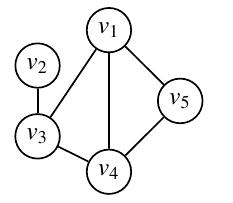
\includegraphics[width=0.3\linewidth]{images/graph18}
\end{figure}
\subsection*{}
La \textbf{coloration} des sommets d'un graphe consiste à affecter à tous les sommets de ce graphe
une couleur de telle sorte que deux sommets adjacents ne portent pas la même couleur. Une
coloration avec $ k $ couleurs est donc une partition de l'ensemble des sommets en $ k $ stables.
Le nombre chromatique du graphe $ G $, noté $ \gamma (G) $, est le plus petit entier $ k $ pour lequel il
existe une partition de $ V $ en $ k $ sous-ensembles stables.
Sur le graphe ci-dessous, on a eu besoin de trois couleurs (notées 1, 2 et 3) pour colorer les
sommets de sorte que deux sommets adjacents aient des couleurs différentes. On a donc
trois stables : $ \{v_{1}, v_{2} \}$, $ \{v_{3}, v_{5}\} $ et $ \{v_{4} \} $. On ne peut pas utiliser moins de couleurs, à cause
des cliques $ \{v_{1},v_{4}, v_{5}\}$ et $ \{v_{1}, v_{3}, v_{4}\} $.

\begin{figure}[h]
\centering
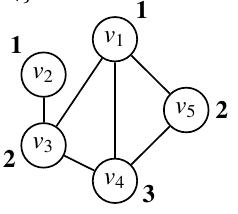
\includegraphics[width=0.3\linewidth]{images/graph19}
\end{figure}

Remarquons enfin que le sommet $ v_{2} $ aurait aussi pu être coloré "3". La coloration minimale n'est donc pas forcément unique.

\subsection*{Encadrement du nombre chromatique}
\subsubsection*{Majoration}
\begin{itemize}
	\item[$\bullet$] $ \gamma (G) \leq r + 1 $, où $ r $ est le plus grand degré des sommets de $ G $.
\textbf{Preuve} : Soit un graphe et $ r $ le degré maximum de ses sommets. Donnons-nous une
palette de $ (r + 1) $ couleurs. Pour chaque sommet du graphe on peut tenir le raisonne-
ment suivant : ce sommet est adjacent à $ r $ sommets au plus, et le nombre de couleurs
déjà utilisées pour colorer ces sommets est donc inférieur ou égal à $ r $ . Il reste donc au
moins une couleur non utilisée dans la palette, avec laquelle nous pouvons colorer notre
sommet.
	\item[$\bullet$] $ \gamma (G) \leq n + 1 - \alpha (G) $
Preuve : Considérons $ S $ un stable de $ V $ de cardinalité $ \alpha (G) $. Une coloration possible
des sommets consiste à colorer les sommets de $ S $ d'une même couleur et les $ n - \alpha (G) $
autres sommets de couleurs toutes différentes. On en déduit que  \\ $ \gamma (G) \leq 1 + (n - \alpha (G)) $.
\end{itemize}

\subsubsection*{Minoration}
\begin{itemize}
\item[$ \bullet$]  Le nombre chromatique d'un graphe est supérieur ou égal à celui de chacun de ses
sous-graphes.
Preuve : Ce résultat découle de la définition même du nombre chromatique.
\item[$ \bullet $] Le nombre chromatique du graphe sera supérieur ou égal à l'ordre de sa plus grande
clique, que l'on note $ \omega (G) $ (prononcer oméga de $ G $). Autrement dit, $ \gamma (G) \geq \omega (G) $
Preuve : Puisque, par définition, dans une clique d'ordre m, tous les sommets sont
adjacents entre eux, il faudra m couleurs. Donc, il faudra au moins $ \omega (G) $ couleurs pour
colorer le graphe $ G $.
\end{itemize}

\subsection*{Algorithme de coloration de Welsh et Powell}
\noindent Cet algorithme couramment utilisé permet d'obtenir une assez bonne coloration d'un
graphe, c'est-à-dire une coloration n'utilisant pas un trop grand nombre de couleurs.
Cependant il n'assure pas que le nombre de couleurs soit minimum (et donc égal au nombre
chromatique du graphe).\\
\textbf{Étape 1}\\
Classer les sommets du graphe dans l'ordre décroissant de leur degré, et attribuer à chacun
des sommets son numéro d'ordre dans la liste obtenue.\\
\textbf{Étape 2}  \\
En parcourant la liste dans l'ordre, attribuer une couleur non encore utilisée au premier
sommet non encore coloré, et attribuer cette même couleur à chaque sommet non encore
coloré et non adjacent à un sommet de cette couleur.\\
\textbf{ Étape 3}  \\
S'il reste des sommets non colorés dans le graphe, revenir à l'étape 2. Sinon, FIN.

\subsection*{Graphes parfaits}
\noindent Dans le cadre de la théorie des graphes, Claude Berge a introduit en 1960 la notion de
\textbf{graphe parfait} comme définissant un graphe pour lequel le nombre chromatique de chaque
sous-graphe induit et la taille de la plus grande clique dudit sous-graphe induit sont égaux.
Un graphe $ G $ est donc parfait si pour tout sous-graphe induit $ G' $ de $ G $ on a $ \gamma (G' ) = \omega (G' ) $.

\subsection*{Coloration des sommets d'un graphe planaire}
\paragraph*{Théorème 1.14 (Théorème des quatre couleurs)}
On peut colorer les sommets d'un graphe planaire (sans boucles) en utilisant au plus
quatre couleurs de telle sorte que toutes les arêtes aient des extrémités de couleurs
différentes.

\paragraph*{$\ \ $}
\noindent Cette conjecture a été formulée pour la première fois par l'Écossais Francis Guthrie en 1852.
Il était alors question de coloration de carte de géographie. La preuve
de ce théorème n'arriva qu'en... 1976, grâce à Kenneth Appel et Wolfgang Haken. La démonstration
 fit grand bruit car ce fut le premier théorème de l'histoire des mathématiques
qui a nécessité l'usage systématique de l'ordinateur.

\subsection*{Coloration des arêtes d'un graphe}
\noindent La coloration des arêtes d'un graphe consiste à affecter à toutes les arêtes de ce graphe une
couleur de telle sorte que deux arêtes adjacentes ne portent pas la même couleur.
\textbf{L'indice chromatique} du graphe $ G $ est le plus petit entier $ k $ pour lequel il existe une
coloration des arêtes ; on le note $ \chi (G) $.
Pour colorer les arêtes d'un graphe, on peut se ramener au problème de la coloration des
sommets. Il suffit pour cela de travailler non pas sur le graphe lui-même, mais sur le graphe
adjoint, noté $ G' $ , et que l'on définit ainsi :
\begin{itemize}
	\item[1.] à chaque arête de $ G = (V, E) $ correspond un sommet de $ G' = (E, F) $
	\item[2.] deux sommets de $ G' $ sont reliés par une arête si les deux arêtes correspondantes de $ G $
sont adjacentes.
\end{itemize}

\begin{figure}[h]
\centering
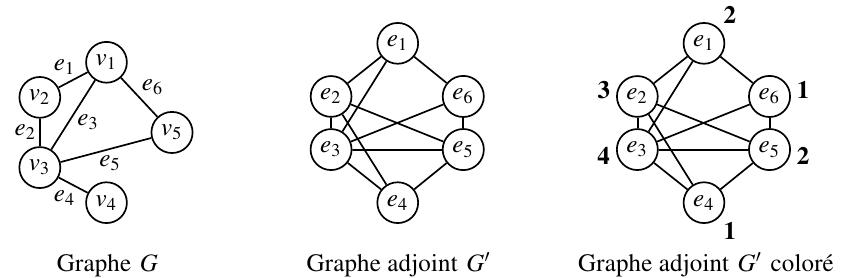
\includegraphics[width=\linewidth]{images/graph20}
\end{figure}

On peut ensuite appliquer l'algorithme de \emph{Welsh} et \emph{Powell} sur le graphe $ G' $ pour colorer
ses sommets. Une fois cela fait, on colorera les arêtes de $ G $ de la même couleur que les
sommets correspondants de $ G' $ .

\subsection{Graphes triangulés}
\noindent Un graphe est \textbf{triangulé} si tous ses cycles de plus de 3 sommets contiennent au moins une
\textbf{corde} (arête reliant deux sommets non adjacents d'un cycle).
Un \textbf{séparateur} est un sous-ensemble $ W $ de sommets dans un graphe connexe $ G = (V, E) $
tel que le graphe $ G[V - W ] $ est non connexe. Dans le graphe ci-dessous, $ W = \{v_{1} , v_{4}\} $ est
un séparateur, $ W = \{v_{3} \}$ est un séparateur minimal.

Un sommet $ v $ est dit \textbf{simplicial} si son voisinage $ N(v) $ est une clique. Dans le graphe ci-dessus, 
les sommets simpliciaux sont $ v_{2} $ et $ v_{5} $ .

\paragraph*{Théorème 1.15}
Un graphe connexe est triangulé si et seulement si tout séparateur minimal est une
clique.

\subsection*{Preuve}
\begin{itemize}
	\item[1.] Supposons tout d'abord que tout séparateur est une clique. Soit $ C = [x_{1} , x_{2}, \dots , x_{k} , x_{1}] $
$ (k \geq 4) $ un cycle dans $ G $ et soit $ W $ un séparateur minimal de $ x_{1} $ et $ x_{3} $ . W doit contenir $ x_{2} $
et au moins un des sommets $ x_{4} ,\dots ,x_{k} $ . Comme W est une clique, il existe une corde
dans $ C $.
\item[2.] Supposons $ G $ triangulé et soit $ W $ un séparateur minimal. Supposons que $ W $ ne soit
pas une clique. Soient $ G_{1} = (V_{1} , E_{1}) $ et $ G_{2} = (V_{2}, E_{2} ) $ deux composantes connexes de
$ G[V-W ] $ et soient $ x $ et $ y $ deux sommets non adjacents dans $ W $ . Comme $ W $ est minimal,
$ x $ et $ y $ ont chacun au moins un voisin dans $ G_{1} $ et dans $ G_{2} $ . Soient $ a_{1} $ et $ a_{2} $ les voisins
de $ x $ dans $ G_{1} $ et $ G_{2} $ , et soient $ b_{1} $ et $ b_{2} $ ceux de y dans $ G_{1} $ et $ G_{2} $ . Comme $ G_{1} $ et $ G_{2}$  $ $
sont connexes, il existe une chaîne reliant a1 à $ b_{1} $ dans $ G_{1} $ et une chaîne reliant $ a_{2} $ à $ b_{2} $
dans $ G_{2} $ . Il existe donc une chaîne $ C_{1} $ sans corde reliant $ x $ à $ y $ dans $ G[V_{1} \bigcup W ] $ ainsi
qu'une chaîne sans corde $ C_{2} $ reliant $ x $ à $ y $ dans $ G[V_{2} \bigcup W ] $. L'union de $ C_{1} $ et $ C_{2} $ est un
cycle sans corde contenant au moins 4 sommets, contradiction.
\end{itemize}

\paragraph*{Théorème 1.16}
Tout graphe triangulé autre qu'une clique contient au moins deux sommets simpliciaux
non adjacents.

\subsection*{Preuve}
Si $ G $ ne contient que deux sommets, alors $ G $ est constitué de deux sommets isolés qui
sont simpliciaux non adjacents. Supposons donc le théorème vrai pour tout graphe ayant
moins de n sommets et soit $ \textbar V \textbar = n $. Soit $ W $ un séparateur minimal et $ G_{1 }= (V_{1} , E_{1}) $
et $ G_{2} = (V_{2}, E_{2} )$ deux composantes connexes de $ G[V - W ] $. On a vu que $ W $ est une clique.
\begin{itemize}
\item Si $ G[V_{1} \bigcup W ] $ est une clique alors choisissons $ x $ dans $ V_{1} $ : $ x $ est simplicial dans $ G[V_{1} \bigcup W ] $.
\item Sinon, par hypothèse d'induction, il existe deux sommets simpliciaux non adjacents dans
\end{itemize}
$ G[V_{1} \bigcup W ] $, et comme $ W $ est une clique, l'un de ces sommets qu'on appellera $ x $ est
dans $ V_{1} $ .
Dans chacun des deux cas on a déterminé un sommet $ x $ simplicial dans $ G[V_{1} \bigcup W ] $. De
même, on peut déterminer un sommet $ y $ simplicial dans $ G[V_{2} \bigcup W ] $. Ces deux sommets $ x $
et $ y $ sont simpliciaux dans $ G $ et non-adjacents.

\subsection*{Algorithme de reconnaissance (Fulkerson et Gross, 1969)}
\begin{itemize}
	\item[1.] Poser $ G' = G $ ;
\item[2.] Si $ G' $ est vide alors $ G $ est triangulé : STOP
\item[3.] Si $ G' $ ne contient pas de sommet simplicial alors G n'est pas triangulé.
\item[4.] Ôter un sommet simplicial de $ G' $ et retourner à 2.
\end{itemize}

Un schéma d'élimination parfait est un ordre $ v_{1} < \dots < v_{n} $ des sommets tel que $ v_{i} $ est
simplicial dans $ G[v_{i} , \dots , v_{n} ] (n = \textbar V \textbar) $.

\paragraph*{Théorème 1.17}
Un graphe est triangulé si et seulement s'il possède un schéma d'élimination parfait.

\subsection*{Preuve}
\noindent \textbf{1.} Soit $ v_{1} < \dots < v_{n} $ un schéma d'élimination parfait et soit $ C = [x_{1} , x_{2}, . . . , x_{k}, x_{1}] (k \geq 4) $
un cycle dans $ G $. Sans perte de généralité, on peut supposer que $  x_{1} = v_{i}$ apparaît avant
$ x_{2}, . . . , x_{k} $ dans le schéma d'élimination parfait. Mais alors $ x_{2} $ est relié à $ x_{k} $ car $ x_{1} $ est
simplicial dans le graphe $ G[v_{i}, \dots , v_{n} ] $ qui contient $ x_{2} , \dots , x_{k} $ . Le cycle $ C $ a donc une
corde.\\
\textbf{2.} Si $ G $ est triangulé on peut déterminer un schéma d'élimination parfait comme suit :
Poser $ i :=1 $ ;
Tant que $ V = \varnothing $ faire\\
Choisir un sommet simplicial $ x $ dans le graphe résiduel. Mettre $ x $ en position $ i $\\
Ôter $ x $ de $ V $ et poser $ i := i + 1 $.

\subsection*{Algorithme de coloration d’un graphe triangulé $ G = (V,E) $}
Déterminer un schéma d’élimination parfait $ v_{1} < \dots < v_{n} $
Colorer $ G $ séquentiellement selon l'ordre inverse $ v_{n} < \dots < v_{1} $ , en utilisant pour chaque
sommet le plus petit numéro de couleur possible.

\section{Graphe orienté}
\subsection{Définition}
\subsection{Graphes orientés}
En donnant un sens aux arêtes d'un graphe, on obtient un digraphe (ou graphe orienté).
Le mot "digraphe" est la contraction de l'expression anglaise "directed graph ".
Un digraphe fini $  G = (V, E) $ est défini par l’ensemble fini $ V = \{v_{1}, v_{2} , \dots , v_{n} \} $ dont 
les éléments sont appelés sommets, et par l'ensemble fini $ E = {e_{1} , e_{2} , . . . , e_{m} } $ dont les éléments
sont appelés arcs.
Un arc e de l'ensemble E est défini par une paire ordonnée de sommets. Lorsque $ e = (u, v) $,
on dit que l'arc $ e $ va de $ u $ à $ v $. On dit aussi que $ u $ est l'extrémité initiale et $ v $ l'extrémité
finale de $ e $.
\subsection{Degré d’un sommet d’un digraphe}
Soit $ v $ un sommet d'un graphe orienté.
On note $ d^{+} (v) $ le degré extérieur du sommet $ v $, c'est-à-dire le nombre d'arcs ayant $ v $
comme extrémité initiale.
On note $ d^{-} (v) $ le degré intérieur du sommet $ v $, c'est-à-dire le nombre d'arcs ayant $ v $
comme extrémité finale.
On définit le degré :
$$ d(v) = d^{ +} (v) + d^{-}(v) $$

\subsection{Chemins et circuits}
Un \textbf{chemin} conduisant du sommet $ a $ au sommet $ b $ est une suite ayant pour éléments alter-
nativement des sommets et des arcs, commençant et se terminant par un sommet, et telle
que chaque arc est encadré à gauche par son sommet origine et à droite par son sommet
destination. On ne peut donc pas prendre les arc à rebours. Sur le digraphe ci-après, on
peut voir par exemple le chemin $ (v_{3}, e_{2 }, v_{2} , e_{1} , v_{1}) $. Par convention, tout chemin comporte
au moins un arc.
On appelle  \textbf{distance}  entre deux sommets d'un digraphe la longueur du plus petit chemin
les reliant. S'il n'existe pas de chemin entre les sommets $ x $ et $ y $, on pose $ d(x, y) = \infty $.
Par exemple, sur le digraphe ci-dessous, $ d(v_{5} , v_{4}) = 2 $, $ d(v_{4}, v_{5}) = \infty $, $ d(v_{3} , v_{1} ) = 1 $,

\begin{figure}[h]
\centering
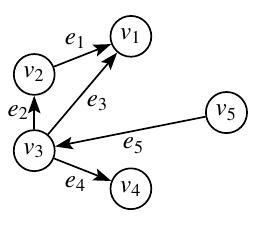
\includegraphics[width=0.4\linewidth]{images/graph22}
\end{figure}

Un \textbf{circuit} est un chemin dont les sommets de départ et de fin sont les mêmes. Le digraphe
ci-dessus ne contient pas de circuit.
Les notions de chemins et de circuits sont analogues à celles des chaînes et des cycles pour
les graphes non orientés.

\subsubsection*{Digraphe fortement connexe}
Un digraphe est \textbf{fortement connexe}, si toute paire ordonnée $ (a, b) $ de sommets distincts du
graphe est reliée par au moins un chemin. En d'autres termes, tout sommet est atteignable
depuis tous les autres sommets par au moins un chemin.
On appelle \textbf{composante fortement connexe} tout sous-graphe induit maximal fortement
connexe (maximal signifie qu'il n'y a pas de sous-graphe induit connexe plus grand contenant les sommets de la composante).


\subsection{Représentations non graphiques des digraphes}
\subsubsection{ Matrice d'adjacences}
On peut représenter un digraphe par une matrice d'adjacences. Une matrice $ (n\times m) $ est
un tableau de $ n $ lignes et $ m $ colonnes. $ (i, j) $ désigne l'intersection de la ligne $ i $ et de la
colonne $ j $ .
Dans une matrice d'adjacences, les lignes et les colonnes représentent les sommets du
graphe. Un "1" à la position $ (i, j ) $ signifie qu'un arc part de $ i $ pour rejoindre $ j $.
\subsection*{Exemple}
Voici la matrice d'adjacences du digraphe G :
\begin{figure}[h]
\centering
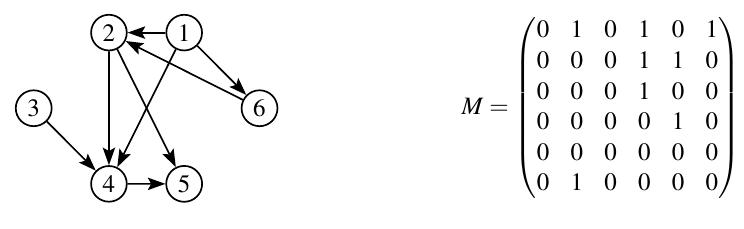
\includegraphics[width=0.7\linewidth]{images/graph23}
\end{figure}

Cette matrice a plusieurs caractéristiques :
\begin{itemize}
	\item[1.] Elle est carrée : il y a autant de lignes que de colonnes.
\item[2.] Il n'y a que des zéros sur la diagonale. Un "1" sur la diagonale indiquerait une
boucle.
\item[3.] Contrairement à celle d'un graphe non orienté, elle n'est pas symétrique.
\item[4.] Une fois que l'on fixe l'ordre des sommets, il existe une matrice d'adjacences unique
pour chaque digraphe. Celle-ci n'est la matrice d'adjacences d'aucun autre digraphe.
\end{itemize}

\subsubsection{ Listes d'adjacences}
On peut aussi représenter un digraphe en donnant pour chacun de ses sommets la liste des
sommets qu'on peut atteindre directement en suivant un arc (dans le sens de la flèche).
\subsection*{Exemple}
Voici les listes d'adjacences du digraphe $  G $ :
\begin{figure}[h]
\centering
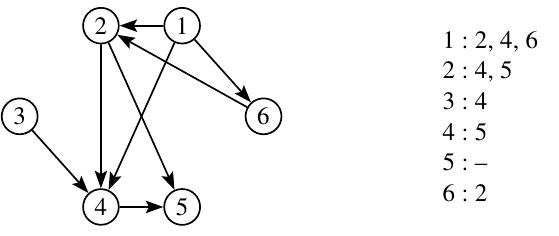
\includegraphics[width=0.6\linewidth]{images/graph24}
\end{figure}

\subsection{Digraphes sans circuit}
\paragraph*{Théorème 2.1}
Le digraphe $ G $ est sans circuit si et seulement si on peut attribuer un nombre $ r(v) $,
appelé le rang de $ v$ , à chaque sommet $ v $ de manière que pour tout arc $ (u, v) $ de $ G$  on ait
$ r(u) < r(v) $.

\subsection*{Preuve}
Si $ G $ comporte un circuit $ C $ , il n'est pas possible de trouver de tels nombres $ r(i) $ car,
autrement, considérant $ r(j) = max\{ r(i) \textbar i \in C\} $ et l'arc $ ( j, k) \in C $ , on aurait $ r(j) \leq r(k) $
en contradiction avec la définition du rang.
Réciproquement, si $ G $ n'a pas de circuit, il existe au moins un sommet sans prédécesseur
dans $ G $ (sans cela, en remontant successivement d'un sommet à un prédécesseur, on finirait
par fermer un circuit). Ainsi, on peut attribuer séquentiellement des valeurs aux sommets
du graphe à l'aide de l'algorithme qui suit, ce qui conclura la démonstration.

\subsection*{Algorithme de calcul du rang}
Donnée : digraphe $ G = (V, E) $ sans circuit.
Résultat : rang $ r(v) $ de chaque sommet $ v \in V $ du digraphe G.

\begin{algorithm}
	\caption{Algorithme de calcul du rang}\label{euclid}
	\begin{algorithmic}[1]
		\Procedure{}{}
		\State $r := 0 $;
		\State $X := V $;
		\State $ R $ : l'ensemble des sommets de $ X $ sans prédécesseur dans $ X $;
		\While {$X\ n'est\ pas\ \varnothing$ }
		\State $ r(v) := r $ pour tout sommet $ v \in R $;
		\State $ X := X - R $;
		\State $ R $ : l'ensemble des sommets de $ X $ sans prédécesseur dans $ X$;
		\State $ r := r + 1$;
		\EndWhile
		\EndProcedure
	\end{algorithmic}
\end{algorithm}

\subsection{Graphes de comparabilité}
Un graphe est de comparabilité si on peut orienter ses arêtes de façon transitive, c'est-à-
dire de telle sorte que s'il existe un arc de i vers j et un arc de j vers k , alors il existe
également un arc de i vers k .

\subsection*{Algorithme permettant de déterminer si G = (V,E) est un graphe de comparabilité}
\noindent \textbf{1.} $ F := \varnothing $\\
\textbf{2.} \textbf{Tant que} $ F = E $ \textbf{faire}\\
Choisir une arête e dans $ E - F  $, donner une orientation à e et compléter cette
orientation pour assurer une orientation transitive de $ G $.\\
\textbf{Si} une arête doit être orientée dans les deux sens,\\ \textbf{STOP} :\\
$ G $ n'est pas de comparabilité.\\
\textbf{Sinon}, rajouter à $ F $ toutes les arêtes nouvellement orientées. Si $ F = E $ \textbf{alors}\\
\textbf{STOP} :
$ G $ est de comparabilité.
\subsection*{Exemple}
\begin{figure}[h]
\centering
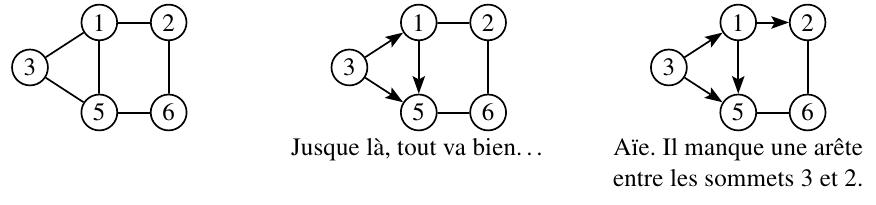
\includegraphics[width=\linewidth]{images/graph25}
\end{figure}
